\documentclass[12pt]{beamer}
\usetheme{Hannover}
\usepackage{graphicx}
\usepackage{booktabs}
\usepackage[english]{babel}
\usepackage{kotex}
%\usepackage[pdfencoding=auto]{hyperref}
\hypersetup{pdfencoding=auto}
\usepackage{ulem}
\usepackage[per-mode=symbol]{siunitx}
\sisetup{inter-unit-product =$\cdot$}
\usepackage{verbatim}
\setbeamertemplate{caption}[numbered]
\graphicspath{{images/}}

\title[\LaTeX - Day 2]{\LaTeX 입문 - Day 2}

\author{14041 박승원}
\institute[GSHS]
{과학영재학교 경기과학고등학교 \TeX 사용자협회 \\ 
\medskip
psw14041@gmail.com (@seungwonpark GitHub)
}
\date{마지막 수정일 : \today}

%\setbeamertemplate{navigation symbols}{}%to suppress navigation tools

\AtBeginSection[]{
	\begin{frame}
		\vfill
		\centering
		\begin{beamercolorbox}[sep=8pt,center,shadow=true,rounded=true]{title}
			\usebeamerfont{title}\insertsectionhead\par%
		\end{beamercolorbox}
		\vfill
	\end{frame}
}
\begin{document}

\begin{frame}
\titlepage % Print the title page as the first slide
\end{frame}

\begin{frame}{지난 시간에는}
	\begin{itemize}
		\item \TeX 소개, 설치, 문서 구조
		\item 수식 입력 방법 및 SI 단위 사용법
		\item 워드프로세서 로서의 \TeX 기본사항
		\item 열거 환경
	\end{itemize}
	이번 시간에는 본격적인 논문 작성 방법에 대해 알아보겠다.
\end{frame}

\section{라벨링 및 상호 참조}
\begin{frame}{라벨링}
	수식\footnote{물론, \$ ... \$ 와 같은 단순한 mathmode 의 수식들은 불가능. equation* 환경과 같이 번호를 매기지 않는 수식도 마찬가지로 불가능하다.}, 그림, 표, 절 모두 라벨링이 가능하며, \textbf{번호가 자동으로 매겨진다.}
	
	라벨링을 할 때는 자신이 기억하기 쉬운 단어를 사용하면 된다. 단, 이 라벨이 수식, 그림, 표, 절인지 구분하지 위해서 라벨은 `eq\_', `fig\_', `tab\_', `sec\_' 와 같이 시작하는 것이 좋다.

	
\end{frame}

\begin{frame}{상호 참조}
	라벨을 참조하려면 \textbackslash ref\{라벨명\} 와 같이 사용하면 된다.
	등식의 경우 \textbackslash eqref\{...\} 를 사용해야 괄호가 쳐진 번호로 나타난다.
	
	예시는 아래와 같다. 코드 : \footnote{\url{http://pastebin.com/4jayE5X0}}
	\begin{figure}
		\centering
		\fbox{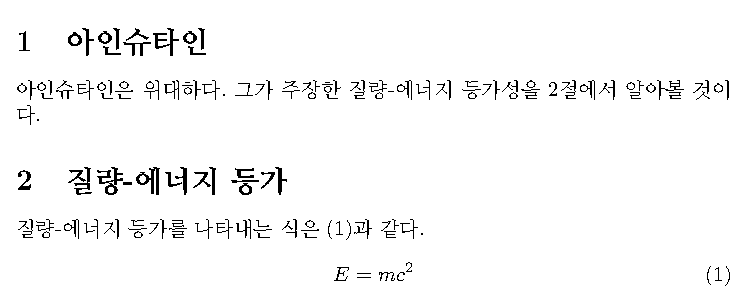
\includegraphics[width=\textwidth]{test_crop_v2.pdf}}
	\end{figure}
\end{frame}
\begin{frame}{자동 조사 기능}
	한글로 논문을 작성할 경우 그림 1과..., 2와..., 와 같이 조사가 바뀌는 경우가 있다. 따라서 `\textbackslash 과', `\textbackslash 와' 와 같이 둘 중 아무 것이나 입력해 놓으면 자동으로 조사가 변경된다. 자동 조사 명령은 다음 12가지가 있다.
	\begin{center}
		\fbox{\small \textbackslash 이 \textbackslash 가, \textbackslash 을 \textbackslash 를, \textbackslash 와 \textbackslash 과, \textbackslash 로 \textbackslash 으로, \textbackslash 은 \textbackslash 는, \textbackslash 라 \textbackslash 이라}
	\end{center}
\end{frame}

\section{떠다니는 개체}

\subsection{그림 삽입}
\begin{frame}[fragile]{그림 삽입 : 기본적인 구조}
	\begin{center}
		\begin{scriptsize}
			\begin{verbatim}
			\begin{figure}[htbp]
			\centering
			\includegraphics[width=.3\textwidth]{example-image-a}
			\caption{Example Image a.}
			\label{fig_example_a}
			\end{figure}
			\end{verbatim}
		\end{scriptsize}
	\end{center}
	결과는 그림 \ref{fig_example_a}\와 같다.
	
	\begin{figure}[htbp]
		\centering
		\includegraphics[width=.3\textwidth]{example-image-a}
		\caption{Example Image a.}
		\label{fig_example_a}
	\end{figure}
\end{frame}
\begin{frame}[fragile]{그림 삽입 코드 설명}
	\begin{center}
		\begin{scriptsize}
			\begin{verbatim}
			\begin{figure}[htbp]
			\centering
			\includegraphics[width=.3\textwidth]{example-image-a}
			\caption{Example Image a.}
			\label{fig_example_a}
			\end{figure}
			\end{verbatim}
		\end{scriptsize}
	\end{center}
	\begin{itemize}
		\item htbp : 다음 슬라이드 참조
		\item \textbackslash centering : 그림의 중앙 정렬
		\item width=.3\textbackslash textwidth : 그림의 크기 = 본문 너비의 0.3배. width 외에도 height, scale을 사용 가능.
		\item example-image-a : 여기에 그림파일 이름을 넣으면 된다. 그림은 지정된 디렉토리\footnote{설정이 없을 경우 .tex 파일과 같은 디렉토리. \textbackslash graphicspath\{\{images/\}\} 와 같이 지정 가능하며, 훨씬 깔끔하다.}에 있으면 된다.
		\item 반드시 \textbf{caption 다음에 label}을 달아야 한다.
	\end{itemize}
\end{frame}
\begin{frame}{h,t,b,p 옵션}
	`\textbackslash begin\{figure\}' 바로 뒤의 대괄호에 등장하는 옵션에 대해 알아보자.
	\begin{table}
		\centering
		\begin{tabular}{|c|p{0.8\textwidth}|}
			\hline
			h & 개체를 코드의 위치(여기 : \textbf{h}ere)에 놓음 \\
			\hline
			t & 개체를 페이지의 맨 위쪽(\textbf{t}op)에 놓음 \\
			\hline
			b & 개체를 페이지의 맨 아래쪽(\textbf{b}ottom)에 놓음 \\
			\hline
			p & 개체를 특정 페이지(\textbf{p}age)에 놓음. 별다른 설정이 없으면 문서의 맨 뒤. \\
			\hline
			! & \LaTeX 에서 미리 설정해놓은 일부 서식을 무시하고(ex. 텍스트 여백) 놓음\\
			\hline
		\end{tabular}
	\end{table}
\end{frame}
\begin{frame}{h,t,b,p 옵션}
	보통의 워드프로세서를 사용하던 것처럼 하려면 단순히 h를 사용하면 된다. 하지만 때로는 h가 불가능하기 때문에, 이미지가 페이지 경계를 넘어간다든지 하는 일을 막으려면 htbp와 같이 차선책을 두어 주는 것이 좋다. tpbh 등으로 설정해도 htbp 순으로 적용된다.
	
	또한, 대부분의 학술지는 두 단으로 나누어진 양식을 채택하는데, 이 경우 그림을 페이지의 중간에 놓는 것보다는 맨 위에 두고, 맨 위에 둘 수 없다면 맨 아래에 두는 것이 좋다. 다음 두 페이지의 예시를 보자.
\end{frame}
\begin{frame}{품위 있는 그림 및 표 배치}
	\begin{figure}[h]
		\centering
		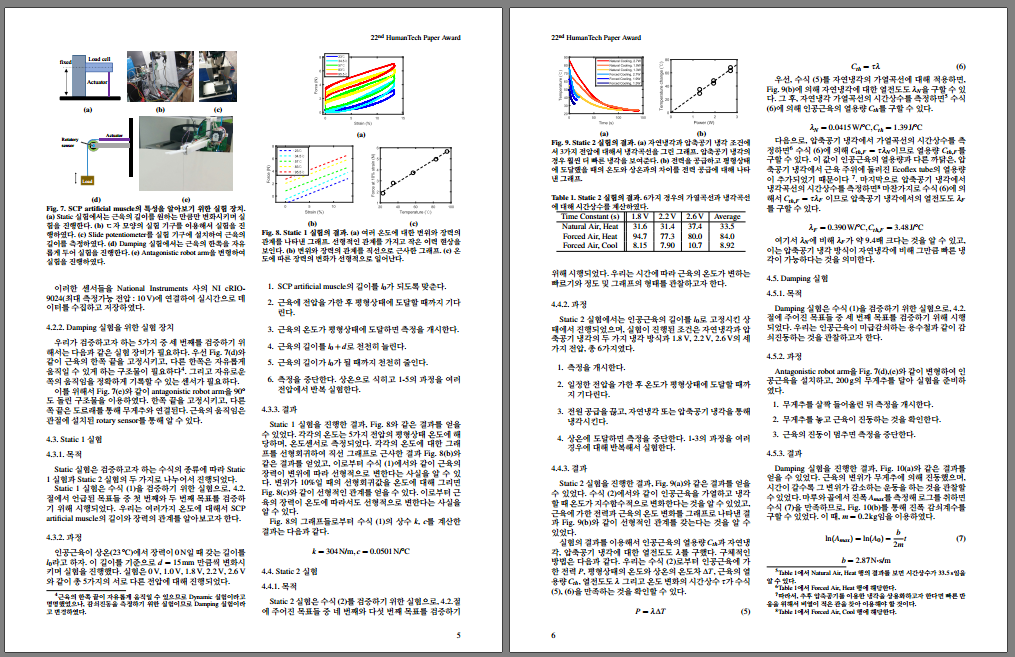
\includegraphics[width=.9\textwidth]{right_fig.png}
	\end{figure}
	\footnote{출처 : 김형주, 박승원, ``SCP Artificial Muscle로 작동하는 Antagonistic Robot Arm의 Feedback 제어''(2015)}
\end{frame}
\begin{frame}{올바르지 못하게 했을 경우}
	
	{\small (같은 논문에서 [t] 옵션을 모두 [h] 로 바꾼 결과이다.)}
	\begin{figure}[h]
		\centering
		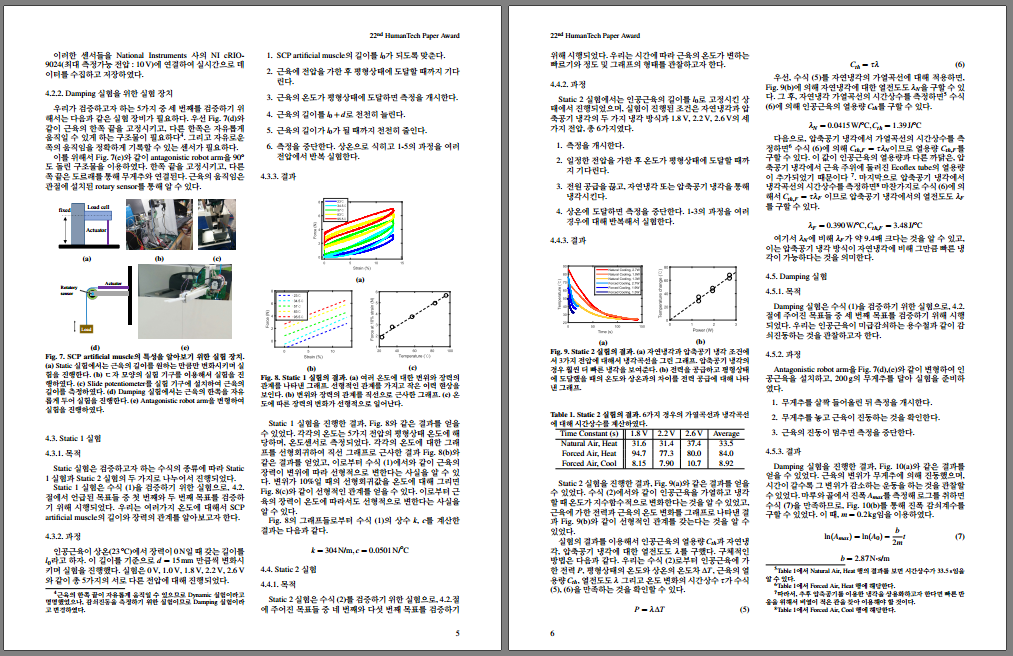
\includegraphics[width=.9\textwidth]{wrong_fig_v2.png}
	\end{figure}
\end{frame}
\begin{frame}{정확한 위치에 놓기}
	다만 때에 따라서는 그림을 정확한 위치에 놓아야 할 때가 있다.
	
	그럴 때는 `float' package의 H 옵션을 사용하자. figure 환경에서 htbp 대신 H를 사용하면 된다.
\end{frame}
\begin{frame}{그림의 유형}
	삽입할 그림의 유형에 대해 적합한 이미지 형식은 다음과 같다.
	\begin{itemize}
		\item 사진 : jpg 또는 jpeg 파일
		\item 그래프 : pdf 또는 eps (벡터 이미지)
		\item 기하적 그림 : png로 캡처 혹은 벡터 이미지
		\item 일러스트 : pdf
	\end{itemize}
	\begin{footnotesize}
		기하적 그림의 경우, GeoGebra에서는 export to tikz 가 되며, standalone class를 이용해 벡터 이미지로 뽑아낼 수 있다. 필요하면 찾아보시길.
		
		일러스트의 경우 보통 PowerPoint로 만든다. `pdf로 내보내기' 기능을 이용하여 .pdf 형식의 벡터 이미지를 얻을 수 있다.
		
		pdf 이미지의 여백이 심할 경우 online pdfcrop 을 찾아보라.
	\end{footnotesize}
\end{frame}
\begin{frame}[fragile]{Subfigure}
	예시 및 코드\footnote{\url{http://pastebin.com/fUSHv8FK}} : 
	\begin{figure}
		\centering
		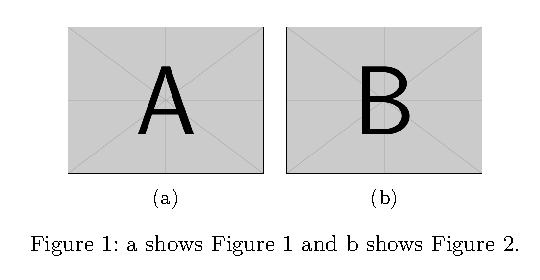
\includegraphics[width=.8\textwidth]{subfigure.pdf}
	\end{figure}
\end{frame}
\subsection{표 삽입}
\begin{frame}[fragile]{표 삽입}
	그림 삽입을 배우고 나면 표는 비교적 간단하다.
	
	인터넷에 latex table generator가 있으니, 이것을 사용하는 것도 꽤 편리하다고 한다. 
	하지만 일단은 설명해 보겠다. 표의 기본적인 구조는 다음과 같다.
	\begin{columns}
		\begin{column}{.4\textwidth}
			\begin{center}
				\begin{scriptsize}
					\begin{verbatim}
					\begin{table}[htbp]
					\centering
					\begin{tabular}{|l|c|r|}
					\hline
					학번&이름&특징\\
					\hline
					\hline
					14041&홍길동&호부호형 못함.\\
					\hline
					14004&전우치&도술에 재능.\\
					\hline
					\end{tabular}
					\end{table}
					\end{verbatim}
				\end{scriptsize}
			\end{center}
		\end{column}
		\begin{column}{.5\textwidth}
			\begin{scriptsize}
				\begin{table}[htbp]
					\centering
					\begin{tabular}{|l|c|r|}
						\hline
						학번&이름&특징\\
						\hline
						\hline
						14200&홍길동&호부호형 못함.\\
						\hline
						14300&전우치&도술에 재능.\\
						\hline
					\end{tabular}
				\end{table}
			\end{scriptsize}
		\end{column}
	\end{columns}
\end{frame}
\begin{frame}{표 작성하기}
	\begin{table}
		\centering
		\begin{tabular}{|c|c|}
			\hline
			l & 좌측 정렬 열 \\
			\hline
			c & 중앙 정렬 열 \\
			\hline
			r & 우측 정렬 열 \\
			\hline
			p\{`width'\} & 폭이 지정된 열. 상측 정렬됨. \\
			\hline
			\textbar & 수직 선(여러 개 사용가능) \\
			\hline
			\& & 열 구분 기호 \\
			\hline
			\textbackslash\textbackslash & 개행 \\
			\hline
			\textbackslash hline & 수평 선(여러 개 사용가능) \\
			\hline
			\textbackslash cline\{i-j\} & i열부터 j열까지의 수평 선 \\
			\hline
		\end{tabular}
	\end{table}
\end{frame}
\begin{frame}{표 예시}
	조금(?) 어려운 표의 예시이다. 보면서 공부하면 도움이 될 것이다.
	코드 : \footnote{\url{http://pastebin.com/1A8L4HjG}}
	\begin{figure}
		\centering
		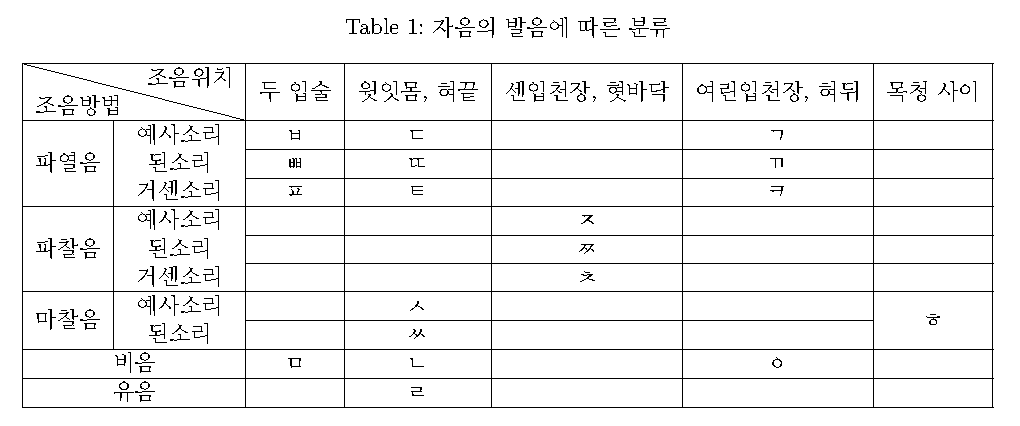
\includegraphics[width=\textwidth]{table_adv.pdf}
	\end{figure}
\end{frame}



\section{논문 작성}
\subsection{문서 계층}
\begin{frame}{문서 계층}
	\begin{figure}
		\centering
		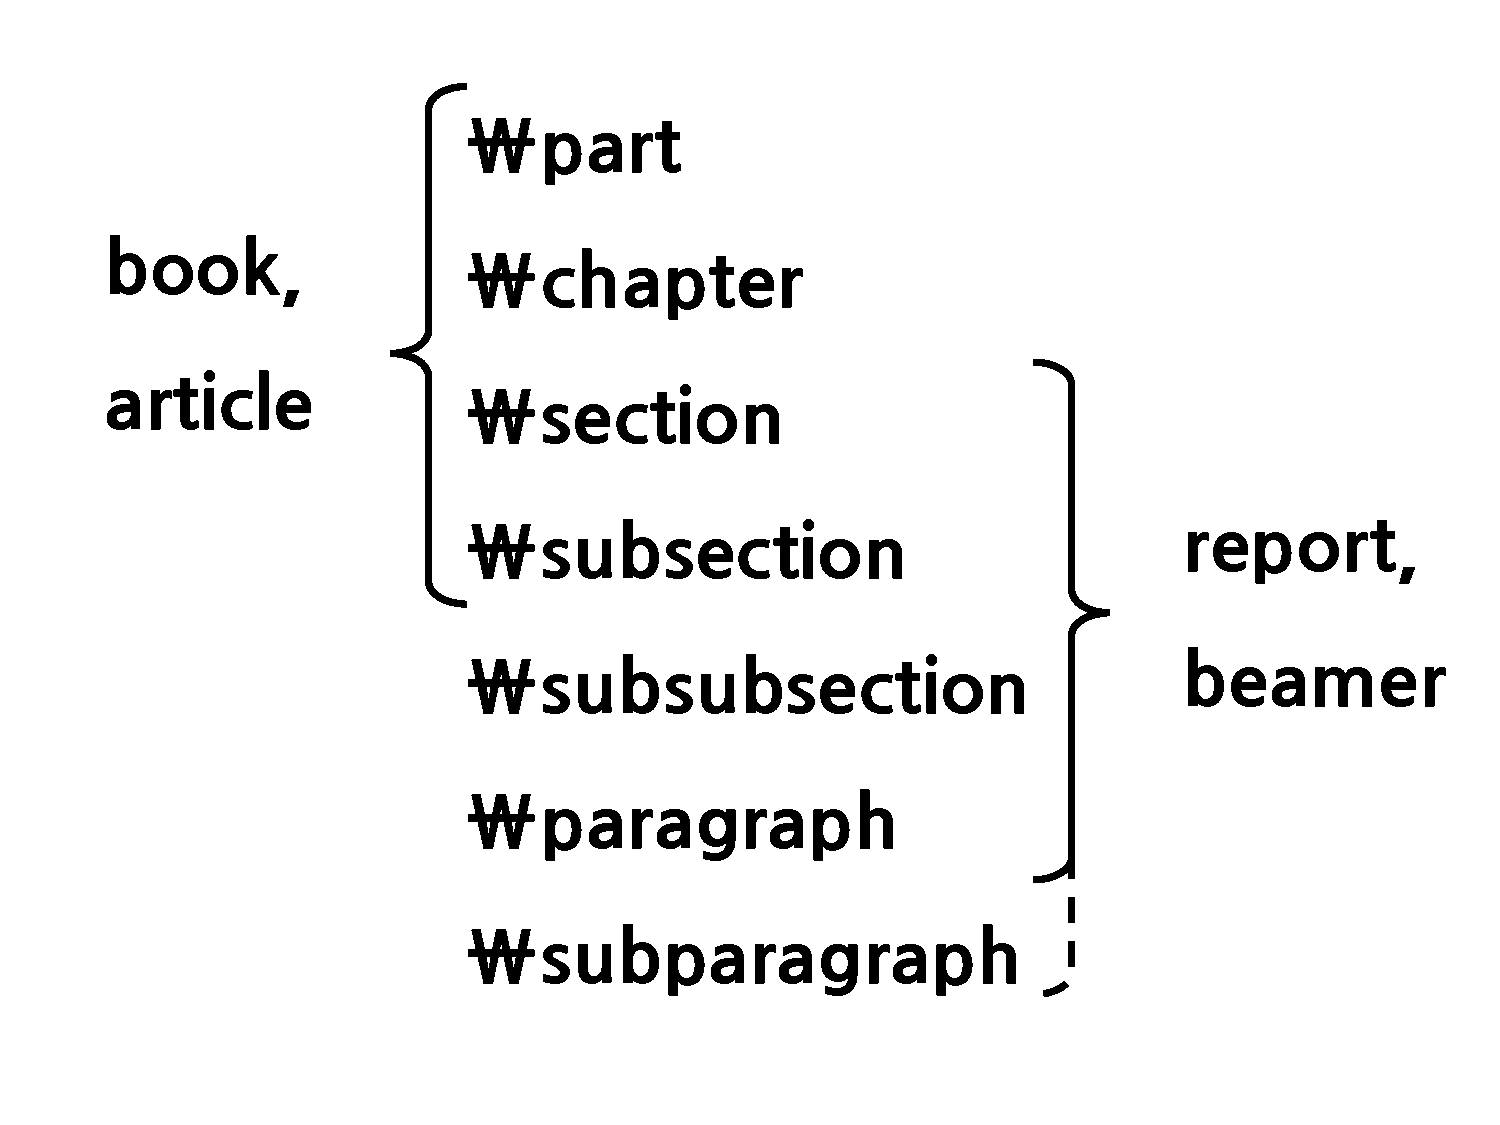
\includegraphics[width=\textwidth]{hier.pdf}
	\end{figure}
\end{frame}
\subsection{참고 문헌 삽입}
\begin{frame}{참고 문헌 삽입}
	졸업논문 양식(이면서도 사용법) 파일에 아주 잘 설명되어 있다. 링크 : \footnote{\url{https://github.com/gshslatexintro/pdf-cloud/raw/master/gshs_thesis_certified_160210.pdf}}
	\vspace{1cm}
	
	참고문헌들은 본문 내에서 반드시 인용되어야 하며, 인용 순으로 정렬되어야 한다. 참고문헌 개수가 많아질 경우 인용 순 정렬이 번거로워지는데, 이럴 땐 BibTeX 을 사용하면 좋다. BibTeX 사용법은 졸업논문 advanced version 에 설명되어 있다. 링크 : \footnote{\url{https://github.com/gshslatexintro/pdf-cloud/raw/master/gshs_thesis_14XXX_main_160422.pdf}}
\end{frame}
\subsection{ToC, LoF, LoT}
\begin{frame}{ToC, LoF, LoT}
	\LaTeX 에 의해 \textbf{자동 생성} 된다! 단, 이들은 컴파일을 2회 해 주어야 갱신된다. \footnote{.tex 파일과 같은 디렉토리 내에 생성되는 .toc, .lof, .lot 파일이 이들이다.}
	\begin{itemize}
		\item Table of Contents : ToC \\
		\textbackslash tableofcontents
		\item List of Figures : LoF
		\textbackslash listoffigures
		\item List of Tables : LoT
		\textbackslash listoftables
	\end{itemize}
	
\end{frame}
\begin{frame}{요약 캡션}
	LoF 와 LoT 에는 해당하는 그림과 표의 번호와 caption 이 함께 나타난다. 하지만, caption이 긴 경우 이것이 LoF/LoT에 그대로 나온다면 복잡하며 미관상 좋지 않다. 이 경우, 그림/표에서 대괄호 안에 요약 캡션을 달아주면 이것만 LoF/LoT 에 표시된다.
	\begin{center}
		\small
		\fbox{\textbackslash caption[LoF/LoT에 표시되는 캡션]\{본문에 나타나는 캡션\}}
	\end{center}
\end{frame}

\section{Extra Tips}
\begin{frame}{Extra Tips}
	\begin{itemize}
		\item \textbf{Ask Google!} (중요)
		\begin{itemize}
			\item `표의 칸에 대각선 어떻게 넣나요?' : \\
			구글 검색 : `latex table diagonal line'
			\item 키워드를 모르겠다면, 횡설수설 검색하다가 키워드를 찾고, 그 키워드로 다시 검색하면 된다.
		\end{itemize}
		\item 중간중간에 컴파일을 해 본다. \\
		수정 사항이 많은데 에러가 발생할 경우, 찾기가 힘들어짐.
		\item 긴 단어를 많이 사용해야 할 경우, newcommand를 통해 하나의 명령어로 만들어 버린다.
	\end{itemize}
	\begin{footnotesize}
		예시 : \textbackslash newcommand\{\textbackslash scp\}\{SCP Artificial Muscle\} 와 같이 지정하고 본문에서 `\textbackslash scp 은...' 라고만 써놓으면 `SCP Artificial Muscle은...' 와 같이 나온다.
	\end{footnotesize}
\end{frame}
\begin{frame}{Extra Tips}
	\begin{itemize}
		\item TeXstudio에서는 원하는 부분만 컴파일 하여 미리 보는 것이 가능하다. 
		
		마우스 오른쪽 버튼 클릭 후 Preview Selection/Parentheses (단축키 Alt+P).
		
		해제는 마우스 버튼 클릭 후 Clear Inline Preview(단축키 없음).
	\end{itemize}
\end{frame}
\begin{frame}{End}
	\begin{itemize}
		\item 이상 두 차례에 걸친 강의는 전공과목을 불문하고 \TeX 을 사용하는 방법에 관한 것이었다.
		\item 전공에 따라 이 문서의 내용 외에도 더 알아야 할 것은 많다. 
		\begin{itemize}
			\item 예를 들어 수학의 경우 theorem 환경을, 정보과학의 경우 verbatim 이나 lstlistings 환경을 사용해야 할 것이다.
		\end{itemize}
		이러한 전공에 따른 세부 내용은 여기에서 다루지 않았다. 이것들은 독자들이 각자 구글링하여 공부해야 하는 부분이다.
		\item 경기과학고 \TeX 사용자협회\footnote{\url{http://gshslatexintro.github.io}}  에는 현재 수학, 물리, 화학 세 분야에 걸친 \TeX 사용자들이 그들의 tex 문서를 공유하고 있으므로 해당 전공자들은 참고할 수 있을 것이다.
	\end{itemize}
\end{frame}
\begin{frame}{Join GitHub!}
	\begin{itemize}
		\item 본 입문서 제작이나 양식 파일들의 수정 및 보완에 참여하고 싶다면 경기과학고 \TeX 사용자협회의 GitHub 그룹에 참여하세요!
		\item \url{github.com/gshslatexintro}
	\end{itemize}
\end{frame}
\end{document}